%        File: latexdoc.tex
%     Created: Friday March 4 12:24:15 2011
% Last Change: Friday March 4 12:24:20 2011
%
\documentclass[letterpaper,12pt]{article}
\usepackage[top=1.0in,bottom=1.0in,left=1.25in,right=1.25in]{geometry}
\usepackage{verbatim}
\usepackage{amssymb}
\usepackage{graphicx}
\usepackage{longtable}
\usepackage{amsfonts}
\usepackage{amsmath}
\usepackage{amsthm}
\usepackage[mathcal]{euscript}
\usepackage{tabularx}
\usepackage{cite}
\usepackage{c++}
\usepackage{tmadd,tmath}
\usepackage[usenames]{color}
\usepackage[
naturalnames = true, 
colorlinks = true, 
linkcolor = black,
anchorcolor = black,
citecolor = black,
menucolor = black,
urlcolor = blue
]{hyperref}

%%---------------------------------------------------------------------------%%
\author{Stuart R. Slattery
  \\ \href{mailto:sslattery@wisc.edu}{\texttt{sslattery@wisc.edu}}
}

\date{\today}
\title{A Spectral Analysis of the Domain Decomposed Adjoint
  Neumann-Ulam Method}
\begin{document}
\maketitle

%%---------------------------------------------------------------------------%%
\begin{abstract}

  The domain decomposed behavior of the adjoint Neumann-Ulam method
  for solving linear operator equations is analyzed using the spectral
  properties of the linear operator. Relationships for the average
  length of the adjoint random walks and the fraction of histories
  leaking from a domain in the decomposition are made with respect to
  the Eigenvalues and other properties of the linear operator. In
  addition, a formal definition of the optical thickness of a domain
  in the decomposition is presented based on the spectral
  analysis. The one-speed, two-dimensional neutron diffusion equation
  is used as a model problem to test the spectral theory for symmetric
  operators. In general, the spectral theory shows good agreement with
  measured computational results.

\end{abstract}

%%---------------------------------------------------------------------------%%
\section{Introduction}
An alternative approach to approximate matrix inversion is to employ
Monte Carlo methods that sample a distribution with an expectation
value equivalent to that of the inverted operator. Such methods have
been in existence for decades with the earliest reference noted here
an enjoyable manuscript published in 1950 by Forsythe and Leibler
\cite{forsythe_matrix_1950}. In their outline, Forsythe and Liebler
in fact credit the creation of this technique to J. Von Neumann and
S.M. Ulam some years earlier than its publication. In 1952 Wasow
provided a more formal explanation of Von Neumann and Ulam's method
\cite{wasow_note_1952} and Hammersley and Handscomb's 1964 monograph
\cite{hammersley_monte_1964} and Spanier and Gelbard's 1969 book
\cite{spanier_monte_1969} present additional detail on a method
adjoint to that described by Neumann and Ulam.

For very large linear systems, two things are likely to occur: a
single compute node does not contain enough memory to hold the entire
problem or a single compute node takes a prohibitively long time to
solve the system. Domain decomposition methods permit the global
computational domain to be subdivided into smaller regions. These
smaller regions require less memory to store and fewer computational
resources to solve as compared to the global problem. Typically, these
smaller regions are then represented separately in individual compute
nodes. Therefore, in order to solve large scale problems with the
adjoint Neumann-Ulam method, we must explore its behavior in a domain
decomposed environment.

For reactor physics Monte Carlo simulations, domain decomposition has
been identified as a key principle in moving forward in high
performance computing
\cite{brunner_comparison_2006,siegel_analysis_2012}. To accomplish
this, we recognize from the literature that stochastic histories must
be transported from domain to domain as the simulation progresses and
they transition to states that are not in the local domain. Because we
have chosen a domain decomposition strategy in a parallel environment,
this means that communication of these histories must occur between
compute nodes owning neighboring pieces of the global domain. We wish
to characterize this communication not only because communication is
in general expensive, but also because nearest-neighbor communication
sequences have poor algorithmic strong scaling
\cite{gropp_high-performance_2001}.

For problems where the linear operator is symmetric, a host of
analytic theories exist based on the Eigenvalue spectrum of the
operator that characterize their behavior in the context of
deterministic linear solvers. Using past work, these theories are
adapted to the domain decomposed adjoint Neumann-Ulam method using the
one-speed, two-dimensional neutron diffusion equation. In this paper
we describe the adjoint Neumann-Ulam method followed by a presentation
and finite difference discretization of the model problem. Using the
linear system generated by this discretization, we use a spectral
theory to generate analytic relations for the Eigenvalues of the
operator based on system parameters. Using the Eigenvalue spectra, we
then build relationships to characterize the transport of random walk
histories in a decomposed domain and compare these analytic results to
numerical experiments conducted with the model problem.

%%---------------------------------------------------------------------------%%
\section{The Adjoint Neumann-Ulam Method}
We seek solutions of the general linear problem in the following form:
\begin{equation}
  \ve{A} \ve{x} = \ve{b}\:,
  \label{eq:linear_problem}
\end{equation}
where $\ve{A} \in \mathbb{R}^{N \times N}$ is a linear operator such
that $\ve{A} : \mathbb{R}^{N} \rightarrow \mathbb{R}^{N}$, $\ve{x} \in
\mathbb{R}^N$ is the solution vector, and $\ve{b} \in \mathbb{R}^N$ is
the forcing term. Choosing the adjoint method Monte Carlo method to
invert the linear operator, we begin by defining the linear system
adjoint to Eq~(\ref{eq:linear_problem}):
\begin{equation}
  \ve{A}^T \ve{y} = \ve{d}\:,
  \label{eq:adjoint_linear_problem}
\end{equation}
where $\ve{y}$ and $\ve{d}$ are the adjoint solution and source
respectively and $\ve{A}^T$ is the adjoint operator.  With this
statement we can then define the split equation:
\begin{equation}
  \ve{y} = \ve{H}^T \ve{y} + \ve{d}\:,
  \label{eq:adjoint_split_system}
\end{equation}
where $\ve{H} = \ve{I} - \ve{A}$ and is defined as the
\textit{iteration matrix}.  Using these definitions, we can derive an
estimator from the adjoint method that will also give the solution
vector, $\ve{x}$. We can acquire the adjoint solution by forming the
Neumann series by writing Eq~(\ref{eq:adjoint_split_system}) as:
\begin{equation}
  \ve{y} = (\ve{I} - \ve{H}^T)^{-1} \ve{d}\:,
  \label{eq:adjoint_split_system_2}
\end{equation}
which in turn yields the Neumann series using the adjoint operator:
\begin{equation}
  \ve{y} = \sum_{k=0}^{\infty} (\ve{H}^T)^k\ve{d}\:.
  \label{eq:adjoint_neumann_series}
\end{equation}
For this series to converge, we require that the spectral radius of
$\ve{H}$ must remain less than 1 as $\ve{H}^T$ contains the same
Eigenvalues and therefore has the same spectral radius. We expand this
summation to again yield a series of transitions that can be
approximated by a Monte Carlo random walk sequence, forming the
Neumann series in reverse order:
\begin{equation}
  y_i = \sum_{k=0}^{\infty}\sum_{i_1}^{N}\sum_{i_2}^{N}\ldots
  \sum_{i_k}^{N}h_{i_k,i_{k-1}}\ldots h_{i_2,i_1} h_{i_1,i} d_{i_k}\:.
  \label{eq:adjoint_neumann_solution}
\end{equation}
We can readily build an estimator for the adjoint solution from this
series expansion, but we instead desire the solution to
Eq~(\ref{eq:linear_problem}). The adjoint estimator can be related to
the solution by defining the following inner product equivalence
\cite{spanier_monte_1969}:
\begin{equation}
  \langle \ve{A}^T \ve{x}, \ve{y} \rangle = \langle \ve{x}, \ve{A}
  \ve{y} \rangle\:.
  \label{eq:adjoint_operator_product}
\end{equation}
From this definition it follows that:
\begin{equation}
  \langle \ve{x}, \ve{d} \rangle = \langle \ve{y}, \ve{b} \rangle\:.
  \label{eq:adjoint_vector_relation}
\end{equation}
Here we have 2 unknowns, $\ve{y}$ and $\ve{d}$, and therefore we
require two constraints to close the system. We use
Eq~(\ref{eq:adjoint_vector_relation}) as the first constraint and as a
second constraint we select:
\begin{equation}
  \ve{d} = \boldsymbol{\delta}_i\:,
  \label{eq:adjoint_second_constraint}
\end{equation}
where the $k^{th}$ component of the vector $\boldsymbol{\delta}_i$ is
the Dirac delta function $\delta_{i_k,i}$. If we apply
Eq~(\ref{eq:adjoint_second_constraint}) to our first constraint
Eq~(\ref{eq:adjoint_vector_relation}), we get the following convenient
outcome:
\begin{equation}
  \langle \ve{y}, \ve{b} \rangle = \langle \ve{x},
  \boldsymbol{\delta}_i \rangle = x_i \:,
  \label{eq:inner_product_constraint}
\end{equation}
meaning that if we compute the inner product of the original source and
the adjoint solution using a delta function source, we recover the
original solution we are looking for. In terms of particle transport, a
delta function source means that this adjoint method is equivalent to
a traditional forward method where tallies are made only in the state
in which the random walk currently resides.

In order to perform the random walks required to approximate the
summation in Eq~(\ref{eq:adjoint_neumann_solution}), probabilities and
weights are generated using the \textit{adjoint Neumann-Ulam
  decomposition} of $\ve{H}$:
\begin{equation}
  \ve{H}^{T} = \ve{P} \circ \ve{W}\:,
  \label{eq:adjoint_neumann_ulam}
\end{equation}
where now we are forming the decomposition with respect to the
transpose of $\ve{H}$. We then build the probability and weight
matrices in the decomposition where probabilities are column-scaled:
\begin{equation}
  p_{ij} = \frac{|h_{ji}|}{\sum_j |h_{ji}|}\:,
  \label{eq:adjoint_probability}
\end{equation}
such that we expect to select a new state $j$ from the current state
in the random walk $j$ by sampling column-wise. Per
Eq~(\ref{eq:adjoint_neumann_ulam}), the transition weight is then
defined as:
\begin{equation}
  w_{ij} = \frac{h_{ji}}{p_{ij}}\:.
  \label{eq:adjoint_weight}
\end{equation}
Using the decomposition we can then define an expectation value for
the adjoint method. Using our result from
Eq~(\ref{eq:inner_product_constraint}) generated by applying the
adjoint constraints, the contribution to the solution in state $i$
from a particular random walk permutation is then:
\begin{equation}
  X_{\nu} = \sum_{m=0}^k W_{m} \delta_{i,i_m}\:,
  \label{eq:adjoint_permutation_contribution}
\end{equation}
where the Kronecker delta indicates that the tally contributes only in
the current state and $b_{i_0}$ will be the sampled source starting
weight. Finally, the expectation value using all permutations is:
\begin{equation}
  E\{X\} = \sum_{\nu} P_{\nu} X_{\nu}\:
  \label{eq:adjoint_expectation_value}
\end{equation}
which if expanded directly recovers the exact solution:
\begin{equation}
  \begin{split}
    E\{X_j\} &=\sum_{k=0}^{\infty}\sum_{i_1}^{N}\sum_{i_2}^{N}\ldots
    \sum_{i_k}^{N} b_{i_0} h_{i_0,i_1}h_{i_1,i_2}\ldots
    h_{i_{k-1},i_k} \delta_{i_k,j} \\ &= x_{j}\:,
  \end{split}
  \label{eq:adjoint_expectation_expansion}
\end{equation}
therefore also providing an unbiased Monte Carlo estimate of the
solution.

We also desire a criteria for random walk termination for problems
where only an approximate solution is necessary. For the adjoint
method, we utilize a relative weight cutoff parameter:
\begin{equation}
  W_f = W_c b_{i_0}\:,
  \label{eq:relative_weight_cutoff}
\end{equation}
where $W_c$ is the \textit{weight cutoff}. The adjoint random
walk will then be terminated after $m$ steps if $W_m < W_f$ as tally
contributions become increasingly small.

%%---------------------------------------------------------------------------%%
\section{Model Problem}
For our numerical experiments, we choose the one-speed,
two-dimensional neutron diffusion equation as a model problem
\cite{duderstadt_nuclear_1976}:
\begin{equation}
  -\boldsymbol{\nabla} \cdot D \boldsymbol{\nabla} \phi + \Sigma_a
  \phi = S\:,
  \label{eq:diffusion_eq}
\end{equation}
where $\phi$ is the neutron flux, $\Sigma_a$ is the absorption cross
section, and $S$ is the source of neutrons. In addition, $D$ is the
diffusion coefficient defined as:
\begin{equation}
  D = \frac{1}{3 ( \Sigma_t - \bar{\mu}\Sigma_s )}\:,
  \label{eq:diffusion_coeff}
\end{equation}
where $\Sigma_s$ is the scattering cross section, $\Sigma_t = \Sigma_a
+ \Sigma_s$ is the total cross section, and $\bar{\mu}$ is the cosine
of the average scattering angle. For simplicity, we will take
$\bar{\mu} = 0$ for our analysis giving $D=(3 \Sigma_t)^{-1}$. In
addition, to further simplify we will assume a homogeneous domain such
that the cross sections remain constant throughout. Doing this permits
us to rewrite Eq~(\ref{eq:diffusion_eq}) as:
\begin{equation}
  -D \boldsymbol{\nabla}^2 \phi + \Sigma_a \phi = S\:.
  \label{eq:diffusion_eq_simple}
\end{equation}

We choose a finite difference scheme on a square Cartesian grid to
discretize the problem. For the Laplacian, we choose the 9-point
stencil shown in Figure~\ref{fig:stencil} over a grid of size $h$
\cite{leveque_finite_2007}:
\begin{multline}
  \nabla^2_9\phi = \frac{1}{6h^2}[4 \phi_{i-1,j} + 4 \phi_{i+1,j}
    + 4 \phi_{i,j-1} + 4 \phi_{i,j+1} + \phi_{i-1,j-1}\\ +
    \phi_{i-1,j+1} + \phi_{i+1,j-1} + \phi_{i+1,j+1} - 20
    \phi_{i,j}]\:.
  \label{eq:nine_point_stencil}
\end{multline}
\begin{figure}[t!]
  \begin{center}
    \scalebox{1.25}{\input{stencil.pdftex_t}}
  \end{center}
  \caption{\textbf{Nine-point Laplacian stencil.}}
  \label{fig:stencil}
\end{figure}
We then have the following linear system to solve:
\begin{multline}
  -\frac{1}{6h^2}[4 \phi_{i-1,j} + 4 \phi_{i+1,j} + 4
    \phi_{i,j-1} + 4 \phi_{i,j+1} + \phi_{i-1,j-1}\\ + \phi_{i-1,j+1}
    + \phi_{i+1,j-1} + \phi_{i+1,j+1} - 20 \phi_{i,j}] + \Sigma_a
  \phi_{i,j} = s_{i,j}\:,
  \label{eq:fd_system}
\end{multline}
and in operator form:
\begin{equation}
  \ve{D}\boldsymbol{\phi}=\ve{s}\:,
  \label{eq:operator_system}
\end{equation}
where $\ve{D}$ is the diffusion operator, $\ve{s}$ is the source in
vector form and $\boldsymbol{\phi}$ is the vector of unknown fluxes.

To close the system, a set of boundary conditions is required. In the
case of a non-reentrant current condition applied to all global
boundaries of the domain, we choose the formulation of Duderstadt by
assuming the flux is zero at some ghost point beyond the
grid. Consider for example the equations on the $i=0$ boundary of the
domain:
\begin{multline}
  -\frac{1}{6h^2}[4 \phi_{-1,j} + 4 \phi_{1,j} + 4 \phi_{0,j-1} +
    4 \phi_{0,j+1} + \phi_{-1,j-1}\\ + \phi_{-1,j+1} + \phi_{1,j-1} +
    \phi_{1,j+1} - 20 \phi_{0,j}] + \Sigma_a \phi_{0,j} = s_{0,j}\:.
  \label{eq:x_min_bnd}
\end{multline}
Here we note some terms where $i=-1$ and therefore are representative
of grid points beyond the boundary of the domain. We set the flux at
these points to be zero, giving a valid set of equations for the $i=0$
boundary:
\begin{multline}
  -\frac{1}{6h^2}[4 \phi_{1,j} + 4 \phi_{0,j-1} + 4 \phi_{0,j+1}
    \\ + \phi_{-1,j+1} + \phi_{1,j-1} + \phi_{1,j+1} - 20 \phi_{0,j}]
  + \Sigma_a \phi_{0,j} = s_{0,j}\:.
  \label{eq:x_min_bnd_2}
\end{multline}
We repeat this procedure for the other boundaries of the domain.

For reflecting boundary conditions, the net current across a boundary
is zero.

%%---------------------------------------------------------------------------%%
\section{Spectral Analysis}
The convergence of the Neumann series in
Eq~(\ref{eq:adjoint_neumann_series}) approximated by the Monte Carlo
solver is dependent on the Eigenvalues of the iteration matrix. In
addition, the Eigenvalues of the linear operator from which the
iteration matrix was derived allow for further analysis of convergence
properties. We will compute the Eigenvalues of these matrices by
assuming Eigenfunctions of the form \cite{leveque_finite_2007}:
\begin{equation}
  \Phi_{p,q}(x,y) = e^{2 \pi \imath p x} e^{2 \pi \imath q y}\:,
  \label{eq:eigenfunction_form}
\end{equation}
where different combinations of $p$ and $q$ represent the different
Eigenmodes of the solution. As these are valid forms of the solution,
then the action of the linear operator on these Eigenfunctions should
give the Eigenvalues of the matrix as they lie on the unit circle in
the complex plane.

\subsection{Diffusion Operator Spectrum}
For the model problem, we first compute the Eigenvalues for the
diffusion operator $\ve{D}$ by applying the operator to the
Eigenfunctions and noting that $x=ih$ and $y=jh$:
\begin{multline}
  \ve{D}\Phi_{p,q}(x,y) = \lambda_{p,q}(\ve{D})
  =\\ -\frac{D}{6h^2}\Big[4 e^{-2 \pi \imath p h} + 4 e^{2 \pi \imath
      p h} + 4 e^{-2 \pi \imath q h} + 4 e^{2 \pi \imath q h} + e^{-2
      \pi \imath p h} e^{-2 \pi \imath q h} \\ + e^{-2 \pi \imath p h}
    e^{2 \pi \imath q h} + e^{2 \pi \imath p h} e^{-2 \pi \imath q h}
    + e^{2 \pi \imath p h} e^{2 \pi \imath q h} - 20\Big] + \Sigma_a
  \:.
  \label{eq:deriv_diff_1}
\end{multline}
Using Euler's formula, we can collapse the exponentials to
trigonometric functions:
\begin{equation}
  \lambda_{p,q}(\ve{D}) = -\frac{D}{6h^2}[ 8 \cos(\pi p h) + 8
    \cos(\pi q h) + 4 \cos(\pi p h) \cos(\pi q h) - 20] + \Sigma_a\:.
  \label{eq:deriv_diff_2}
\end{equation}

As Eq~(\ref{eq:diffusion_eq}) is diagonally dominant, Jacobi
preconditioning is sufficient to reduce the spectral radius of the
iteration matrix below unity and therefore ensure convergence of the
Neumann series. The preconditioner in this case is then $\ve{M} =
diag(\ve{D})$ such that we are solving the following linear system:
\begin{equation}
  \ve{M}^{-1} \ve{D} \boldsymbol{\phi} = \ve{M}^{-1} \ve{s}\:.
  \label{eq:precond_diffsion}
\end{equation}
The operator $\ve{M}^{-1} \ve{D}$ is merely the original diffusion
operator with each row scaled by the diagonal component. As we have
defined a homogeneous domain, the scaling factor is the same for all
rows in the operator. This scaling factor, $\alpha$, is then defined
as the $\phi_{i,j}$ coefficient from Eq~(\ref{eq:fd_system}):
\begin{equation}
  \alpha = \Bigg[\frac{10 D}{3 h^2} + \Sigma_a\Bigg]^{-1}\:.
  \label{eq:jacobi_scaling}
\end{equation}
Using this coefficient, we then have the following spectrum of
preconditioned Eigenvalues:
\begin{equation}
  \lambda_{p,q}(\ve{M}^{-1} \ve{D}) = \alpha \lambda_{p,q}(\ve{D})\:.
  \label{eq:preconditioned_Eigenvalues}
\end{equation}

A good measure of how well-conditioned is a linear system can be
obtained by computing the condition number for the linear operator
defined as:
\begin{equation}
  \kappa(\ve{A}) = ||\ve{A}||\ ||\ve{A}^{-1}||\:,
  \label{eq:condition_number}
\end{equation}
which can be related to the Eigenvalues of the operator as:
\begin{equation}
  \kappa(\ve{A}) =
  \frac{\max_{p,q}\lambda_{p,q}(\ve{A})}{\min_{p,q}\lambda_{p,q}(\ve{A})}\:.
  \label{eq:condition_number_2}
\end{equation}
To compute the condition number for the preconditioned diffusion
system, we must therefore compute the minimum and maximum Eigenvalues
of the diffusion operator. Per Leveque's text
\cite{leveque_finite_2007}, we expect to find these minimum and
maximum Eigenvalues when $p=q$. To find these values,
Eq~(\ref{eq:preconditioned_Eigenvalues}) is plotted as a function of
$p$ with $p=q$ in Figure~\ref{fig:diffusion_spectrum} for various
values of $\Sigma_a$.
\begin{figure}[t!]
  \begin{center}
    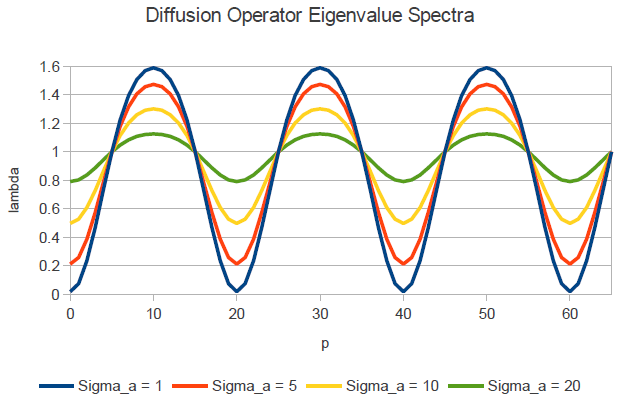
\includegraphics[width=5in,clip]{diffusion_spectrum.png}
  \end{center}
  \caption{\textbf{Eigenvalue spectra for the diffusion equation.}}
  \label{fig:diffusion_spectrum}
\end{figure}
We see a minimum Eigenvalue at $p=0$ and a maximum at $p=10$, letting
us compute the condition number for the Jacobi preconditioned
diffusion operator:
\begin{equation}
  \kappa(\ve{M}^{-1} \ve{D}) =
  \frac{\frac{D}{6h^2}\Sigma_a}{\frac{D}{3h^2}[8 \cos(10 \pi h) + 2
      \cos^2(10 \pi h) - 10] + \Sigma_a}\:.
  \label{eq:diffusion_condition}
\end{equation}
Visually we can also see how increasing the absorption in the problem
creates a more well conditioned system as less diffusion is
expected. If we have a problem with only scattering, $\Sigma_a = 0$
and we observe an infinite condition number as $\lambda_{min}
\rightarrow 0$.

\subsection{Iteration Matrix Spectrum}
The spectral radius of the iteration matrix is obtained by seeking its
largest Eigenvalue. As with the diffusion operator, we can use the
same analysis techniques to find the Eigenvalues for the iteration
matrix. We use a few simplifications by noting that if the Jacobi
preconditioned iteration matrix is $\ve{H} = \ve{I} -
\ve{M}^{-1}\ve{D}$, the we except all terms on the diagonal of the
iteration matrix to be zero such that we have the following stencil:
\begin{equation}
  \ve{H}\boldsymbol{\phi} = -\frac{\alpha D}{6h^2}[4 \phi_{i-1,j}
    + 4 \phi_{i+1,j} + 4 \phi_{i,j-1} + 4 \phi_{i,j+1} +
    \phi_{i-1,j-1}\\ + \phi_{i-1,j+1} + \phi_{i+1,j-1} +
    \phi_{i+1,j+1}]\:.
  \label{eq:iteration_stencil}
\end{equation}
Inserting the Eigenfunctions defined by Eq~\ref{eq:eigenfunction_form}
we get:
\begin{multline}
  \lambda_{p,q}(\ve{H}) = -\frac{\alpha D}{6h^2}\Big[4 e^{-2 \pi \imath p
      h} + 4 e^{2 \pi \imath p h} + 4 e^{-2 \pi \imath q h} + 4 e^{2
      \pi \imath q h} + e^{-2 \pi \imath p h} e^{-2 \pi \imath q h}
    \\ + e^{-2 \pi \imath p h} e^{2 \pi \imath q q} + e^{2 \pi \imath
      p h} e^{-2 \pi \imath q h} + e^{2 \pi \imath p h} e^{2 \pi
      \imath q h}\Big]\:,
  \label{eq:iteration_deriv}
\end{multline}
which simplifies to:
\begin{equation}
  \lambda_{p,q}(\ve{H}) = -\frac{\alpha D}{6h^2}[ 8 \cos(\pi p h) + 8
    \cos(\pi q h) + 4 \cos(\pi p h) \cos(\pi q h)]\:,
  \label{eq:iteration_spectrum}
\end{equation}
giving the Eigenvalue spectrum for the Jacobi preconditioned iteration
matrix. As with the linear operator, we expect the maximum Eigenvalue
to exist when $p=q$. In addition, we note that we have the same cosine
form of the spectrum as for the linear operator expect that the
spectra will be shifted by 10 in the $-p$ direction. We therefore
expect the maximum Eigenvalues to be found when $p=q=0$, giving the
following for the spectral radius of the Jacobi preconditioned
iteration matrix:
\begin{equation}
  \rho(\ve{H}) = \frac{10 \alpha D}{3 h^2}\:.
  \label{eq:iteration_radius}
\end{equation}

\subsection{Neumann Series Convergence}
The Neumann-Ulam method for matrix inversion is effectively an
approximation to a stationary method (the Jacobi method in the case of
the preconditioning above). Stationary methods for linear systems
arise from splitting the operator in Eq~(\ref{eq:linear_problem}):
\begin{equation}
  \ve{A} = \ve{M} - \ve{N}\:,
  \label{eq:split_linear_operator}
\end{equation}
where the choice of $\ve{M}$ and $\ve{N}$ will be dictated by the
particular method chosen. Using this split definition of the operator
we can then write:
\begin{equation}
  \ve{M}\ve{x} - \ve{N}\ve{x} = \ve{b}\:.
  \label{eq:linear_split_equation1}
\end{equation}
By rearranging, we can generate a form more useful for analysis:
\begin{equation}
  \ve{x} = \ve{H}\ve{x} + \ve{c}\:,
  \label{eq:linear_split_equation2}
\end{equation}
where $\ve{H}=\ve{M}^{-1}\ve{N}$ is again defined as the iteration
matrix and $\ve{c}=\ve{M}^{-1}\ve{b}$. With the solution vector on
both the left and right hand sides, an iterative method can then be
formed:
\begin{equation}
  \ve{x}^{k+1} = \ve{H}\ve{x}^k + \ve{c}\:,
  \label{eq:linear_iterative_method}
\end{equation}
with $k \in \mathbb{Z}^+$ defined as the \textit{iteration
  index}. Given this, we can then generate a few statements regarding
the convergence of such stationary methods. Defining $\ve{e}^k =
\ve{u}^k - \ve{u}$ as the solution error at the $k^{th}$ iterate, we
can subtract Eq~(\ref{eq:linear_split_equation2}) from
Eq~(\ref{eq:linear_iterative_method}) to arrive at an error form of
the linear problem:
\begin{equation}
  \ve{e}^{k+1} = \ve{H}\ve{e}^k\:. 
  \label{eq:linear_iterative_error}
\end{equation}
Our error after $k$ iterations is then:
\begin{equation}
  \ve{e}^{k} = \ve{H}^k\ve{e}^0\:. 
  \label{eq:linear_k_iter_error}
\end{equation}
In other words, successive application of the iteration matrix is the
mechanism driving down the error in a stationary method. We can then
place restrictions on the iteration matrix by assuming $\ve{H}$ is
diagonalizable \cite{saad_iterative_2003}, we then have:
\begin{equation}
  \ve{e}^{k} =
  \ve{R}\boldsymbol{\Lambda}^k\ve{R}^{-1}\ve{e}^0\:,
  \label{eq:linear_k_iter_error_diag}
\end{equation}
where $\boldsymbol{\Lambda}$ contains the Eigenvalues of $\ve{H}$ on
its diagonal and the columns of $\ve{R}$ contain the Eigenvectors of
$\ve{H}$. Computing the 2-norm of the above form then gives:
\begin{equation}
  ||\ve{e}^{k}||_2 \leq ||\boldsymbol{\Lambda}^k||_2\ 
  ||\ve{R}||_2\ ||\ve{R}^{-1}||_2\ ||\ve{e}^0||_2\:,
  \label{eq:linear_k_iter_norm1}
\end{equation}
which gives:
\begin{equation}
  ||\ve{e}^{k}||_2 \leq \rho(\ve{H})^k \kappa(\ve{R})
  ||\ve{e}^0||_2\:.
  \label{eq:linear_k_iter_norm2}
\end{equation}
For iteration matrices where the Eigenvectors are orthogonal,
$\kappa(\ve{R})=1$ and the error bound reduces to:
\begin{equation}
  ||\ve{e}^{k}||_2 \leq \rho(\ve{H})^k ||\ve{e}^0||_2\:.
  \label{eq:linear_k_iter_norm3}
\end{equation}
We can now restrict $\ve{H}$ by asserting that $\rho(\ve{H}) < 1$
for a stationary method to converge such that $k$ applications of the
iteration matrix will not cause the error to grow in
Eq~(\ref{eq:linear_k_iter_norm3}). 

In the adjoint Neumann-Ulam method, $k$ iterations, equivalent to $k$
applications of the iteration matrix, are approximated by a random
walk of average length $k$ to yield the summation in
Eq~(\ref{eq:adjoint_neumann_solution})
\cite{dimov_new_1998,halton_sequential_1994,danilov_asymptotic_2000}. This
random walk length, or the number of transitions before the
termination of a history (either by the weight cutoff, absorption, or
exiting the domain) is therefore bound to the number of stationary
iterations required to converge to the specified tolerance. In the
case of the adjoint Neumann-Ulam method, no such tolerance exists,
however, we have specified a weight cutoff $W_c$ under which
low-weight histories will be prematurely terminated as their
contributions are deemed minute. After $k$ iterations, a stationary
method is terminated as the error has reached some fraction,
$\epsilon$, of the initial error:
\begin{equation}
  ||\ve{e}^{k}||_2 = \epsilon ||\ve{e}^0||_2\:.
  \label{eq:linear_k_iter_norm4}
\end{equation}
Per Eq~(\ref{eq:linear_k_iter_norm3}), we see that this fraction is
equivalent to $\epsilon = \rho(\ve{H})^k$. For the adjoint Neumann-Ulam
method, if we take this fraction to be the weight cutoff, a measure of
how accurately the contributions of a particular history to the
solution are tallied, we then have the following empirical relation
for $k$:
\begin{equation}
  k = \frac{ \log(W_c) }{ \log( \rho(\ve{H}) ) }\:.
  \label{eq:analytic_k}
\end{equation}
This then gives us a means to estimate the length of the random walks
that will be generated from a particular linear operator based on the
Eigenvalues of its iteration matrix (independent of the linear
operator splitting chosen) and based on the weight cutoff parameter
used in the Neumann-Ulam method

\subsection{Domain Leakage Approximations}
In a domain decomposed situation, not all histories will remain within
the domain they started in and must instead be communicated. This
communication, expected to be expensive, was analyzed by Siegel and
colleagues for idealized, load balanced situations for full nuclear
reactor core Monte Carlo simulations \cite{siegel_analysis_2012}.  To
quantify the number of particles that leak out of the local domain
they define a leakage fraction, $\Lambda$, as:
\begin{equation}
  \Lambda = \frac{average\ \#\ of\ particles\ leaving\ local\ domain}
          {total\ of\ \#\ of\ particles\ starting\ in\ local\ domain}\:.
  \label{eq:leakage_fraction}
\end{equation}
For their studies, they assumed that the value of $\Lambda$ was
dependent on the total cross section of the system via the Wigner
rational approximation. This approximation was developed by Wigner to
compute the neutron leakage probability from the fuel in a reactor as
a simple interpolation between the small and large fuel lump cases,
approximately characterizing the leakage behavior of many common
geometries \cite{duderstadt_nuclear_1976}. 

Outlined more thoroughly by Hwang's chapter in
\cite{azmy_nuclear_2010}, we begin the derivation of Wigner's
approximation by defining $l$ to be the average chord length across
the domain, and $\Sigma_t$ to be the total cross section in the
domain. We then bound the behavior for the leakage fraction in terms
of the optical thickness, $\Sigma_t l$, of the local domain. In the
case of a small domain or a small cross section (and therefore small
probability of absorption or scatter), $\Sigma_t l \rightarrow 0,
\Lambda \rightarrow 1$. For a large domain or large cross section,
$\Sigma_t l \rightarrow \infty, \Lambda \rightarrow (\Sigma_t
l)^{-1}$, where $(\Sigma_t l)^{-1}$ is effectively the number of
interactions that will occur over the length of the chord. Using
Wigner's simple interpolation, we then have a simple formula for the
domain leakage, $\Lambda = 1/(1+\Sigma_t l)$. This provides a leakage
estimate, valid over the entire range of $\Sigma_t l$, in terms of the
optical thickness of the system. In addition to Wigner's
approximation, Hwang also defines the mean-chord approximation based
on the same numerical limits with $\Lambda = (1-e^{-\Sigma_t
  l})/\Sigma_t l$.

In the case of domain decomposed linear operator equations, we can use
diffusion theory to estimate the optical thickness of a domain in the
decomposition and the corresponding leakage fraction in terms of
properties of the linear operator and the discretization. To begin we
must first calculate the mean distance a Monte Carlo history will move
in the grid by computing the mean squared distance of its movement
along the chord defined across the domain of length $l$. After a
single transition a history will have moved a mean squared distance
of:
\begin{equation}
  \langle \bar{r_1^2} \rangle = (n_s h)^2\:,
  \label{eq:step_1_length}
\end{equation}
where $h$ is the size of the grid along the chord and $n_s$ is the
number of grid elements a history will move on average every
transition. For our diffusion model problem, $n_s$ would equate to the
number of states in the $i$ (or $j$ as the problem is symmetric)
direction that a history could potentially move in a single transition
and is dependent on the stencil used for the discretization. After $k$
transitions in the random walk, the history will have moved a mean
squared distance of:
\begin{equation}
  \langle \bar{r_k^2} \rangle = k (n_s h)^2\:.
  \label{eq:step_k_length}
\end{equation}
If our our chord is of length $l$ and there are $n_i$ grid points (or
states to which a history may transition) along that chord, then $h =
l / n_i$ giving:
\begin{equation}
  \langle \bar{r_k^2} \rangle = k \Bigg(\frac{n_s l}{n_i}\Bigg)^2\:.
  \label{eq:step_k_length_sub}
\end{equation}
From diffusion theory, we expect the average number of interactions
along the chord to be:
\begin{equation}
  \tau = \frac{l}{2 d \sqrt{\langle \bar{r_k^2} \rangle}}\:,
  \label{eq:optical_thickness_1}
\end{equation}
where $d$ is the dimension of the problem and $\sqrt{\langle
  \bar{r_k^2} \rangle}$ is effectively the mean free path of the Monte
Carlo history in the domain. We can readily interperet $\tau$ to be
the \textit{effective optical thickness} of the domain of length
$l$. Inserting Eq~(\ref{eq:step_k_length_sub}) we arrive at:
\begin{equation}
  \tau = \frac{n_i}{2 d n_s \sqrt{k}}\:,
  \label{eq:optical_thickness_2}
\end{equation}
which if expanded with Eq~(\ref{eq:analytic_k}) gives us the final
relation for the effective optical thickness:
\begin{equation}
  \tau = \frac{n_i}{2 d n_s}
  \sqrt{\frac{\log(\rho(\ve{H}))}{\log(W_c)}}\:.
  \label{eq:optical_thickness_3}
\end{equation}

Using this optical thickness, we can then complete the leakage
approximations by defining the bounds of $\tau \rightarrow 0, \Lambda
\rightarrow 1$ and $\tau \rightarrow \infty, \Lambda \rightarrow
\tau^{-1}$. We expect this behavior as optically thin domains will
communicate most of their histories while optically thick domains will
leak the fraction of histories that did not interact within. With
these bounds, we can then define the leakage fraction out of a domain
for the adjoint Neumann-Ulam method using the Wigner rational
approximation:
\begin{equation}
  \Lambda = \frac{1}{1+\tau}\:,
  \label{eq:wigner_domain_leakage}
\end{equation}
and using the mean-chord approximation:
\begin{equation}
  \Lambda = \frac{1-e^{-\tau}}{\tau}\:.
  \label{eq:mean_chord_domain_leakage}
\end{equation}
Here, the leakage fraction is explicitly bound to the Eigenvalues of
the iteration matrix, the size of the domain, the content of the
discretization stencil, and the weight cutoff selected to terminate
low weight histories.  We also note here an interesting consequence of
this approximation: no matter how optically thick a domain may be, the
domain is still expected to leak some histories and thus communicate
them. Therefore, no matter how large the domains are made, if they do
not encapsulate the entire global domain they require some
communication in order to implement a domain decomposed adjoint
Neumann-Ulam method.

%%---------------------------------------------------------------------------%%
\section{Numerical Experiments}
To test the relationships developed by the spectral analysis, we form
two simple numerical experiments using the diffusion model problem:
one to measure the length of the random walks as a function of the
iteration matrix Eigenvalues, and one to measure the domain leakage
fraction as a function of the iteration matrix Eigenvalues and the
discretization properties. Before doing this, we verify our
computation of the spectral radius of the iteration matrix by
numerically computing the largest Eigenvalue of the diffusion operator
using an iterative Eigenvalue solver. For this verification, a $100
\times 100$ square grid with $h=0.01$, $h=0.1$, and $h=1.0$ and
non-reentrant current boundary conditions was used and the absorption
cross varied from 0 to 100 while the scattering cross section was
fixed at unity. Figure~\ref{fig:measured_spec_rad} gives the measured
spectral radius of the iteration matrix and the computed spectral
radius for the preconditioned diffusion operator using
Eq~(\ref{eq:iteration_radius}) as function of the absorption to
scattering ratio $(\Sigma_a / \Sigma_s)$. Excellent agreement was
observed between the analytic and numerical results with all data
points computed within the tolerance of the iterative Eigenvalue
solver.
\begin{figure}[t!]
  \begin{center}
    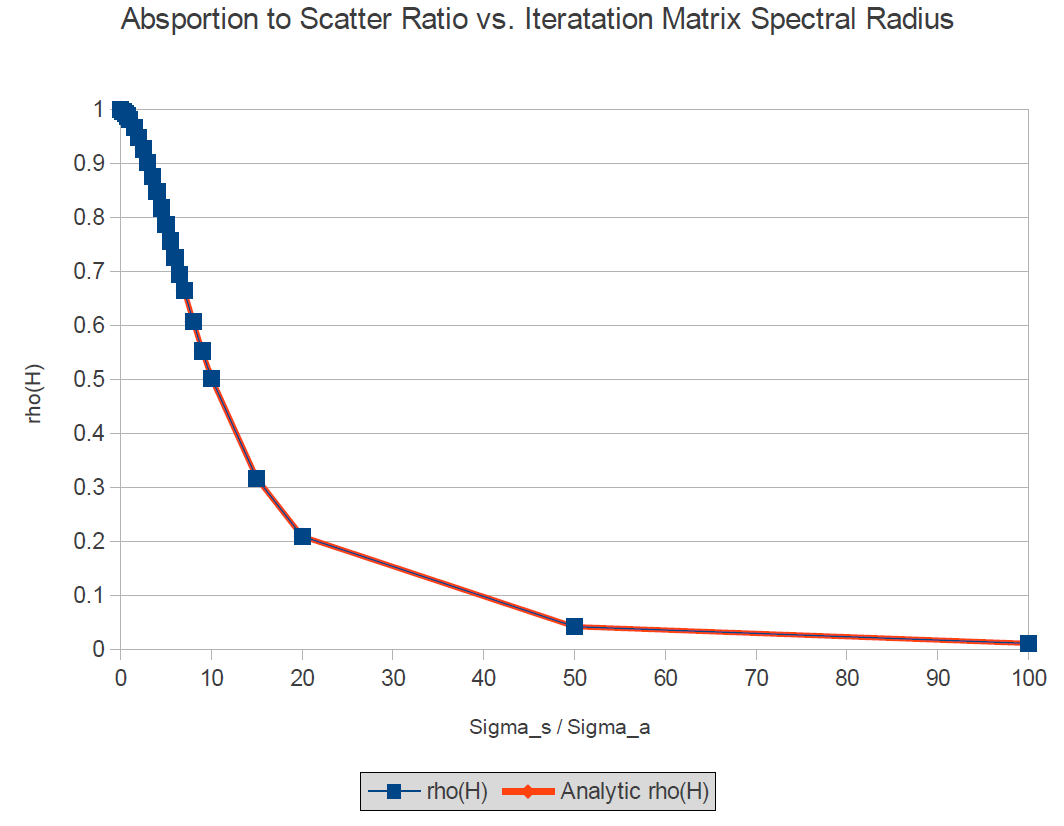
\includegraphics[width=5in,clip]{measured_spec_rad.png}
  \end{center}
  \caption{\textbf{Measured and analytic preconditioned diffusion
      operator spectral radius as a function of the absorption cross
      section to scattering cross section ratio.} \textit{Values of
      $h=0.01$, $h=0.1$, and $h=1.0$ were used to verify the
      behavior. The red data was computed numerically by an
      Eigensolver while the black dashed data was generated by
      Eq~(\ref{eq:iteration_radius}).}}
  \label{fig:measured_spec_rad}
\end{figure}

\subsection{Random Walk Length}
With the spectral data in hand, we can go about setting up an
experiment to measure the length of the random walks generated by the
adjoint Neumann-Ulam solver. To do this, we again use a $100 \times
100$ square grid with $h=0.1$ and non-reentrant current boundary
conditions was used and the absorption cross varied from 0 to 100
while the scattering cross section was fixed at unity. Three weight
cutoff values of \sn{1}{-2}, \sn{1}{-4}, and \sn{1}{-8} were used with
10,000 histories generated by a point source source of strength 1 in
the center of the domain such that the vacuum boundary conditions will
have less of an effect on the length of the random walks. For each of
the histories, the number of transitions made was tallied to provide
an effective value of $k$ for each history. This value was then
averaged over all histories to get a measured value of $k$ for the
particular operator. Figure~\ref{fig:measured_length} gives these
measurements as well as the analytic result computed by
Eq~(\ref{eq:analytic_k}) as a function of the iteration matrix
spectral radius, $\rho(\ve{H})$. Again, we note good agreement between
the measured and analytic results.
\begin{figure}[t!]
  \begin{center}
    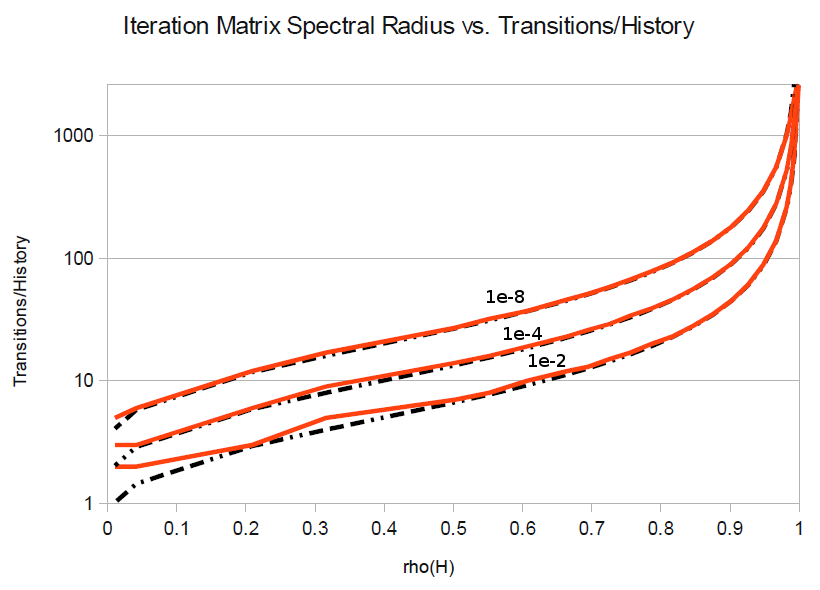
\includegraphics[width=5in,clip]{measured_length.png}
  \end{center}
  \caption{\textbf{Measured and analytic random walk length as a
      function of the iteration matrix spectral radius.} \textit{The
      weight cutoff was varied with \sn{1}{-2}, \sn{1}{-4}, and
      \sn{1}{-8}, to verify the validity of that parameter in
      Eq~(\ref{eq:analytic_k}). The red data was computed numerically
      by an adjoint Neumann-Ulam implementation while the black dashed
      data was generated by Eq~(\ref{eq:analytic_k}).}}
  \label{fig:measured_length}
\end{figure}

\subsection{Domain Leakage}
Finally, we seek to measure the leakage from a domain in a domain
decomposed Monte Carlo calculation and assess the quality of our
analytic relation for the optical thickness of domain and the
associated leakage approximations. For this experiment, square grid
with $h=0.1$ and non-reentrant current boundary conditions. The grid
is then decomposed into 9 square domains, 3 in each cardinal
direction. For the cross sections, the absorption cross was varied
from 1 to 100 while the scattering cross section was set to zero to
create a purely absorbing environment. The optical thickness of these
domains will vary as a function of the absorption cross section if the
other parameters are fixed. To compute the optical thickness, along
with the spectral radius as given by Eq~(\ref{eq:iteration_radius}),
we also need the parameters $n_i$ and $n_s$ which respectively
describe the typical domain length and the average number of states
moved along that typical length per history transition. For our grid
above, the domains are varied in size with $50 \times 50$, $100 \times
100$, and $200 \times 200$ cells giving $n_i=50$, $n_i=100$, and
$n_i=200$ grid points or states along the typical length of the domain
respectively. Looking at the Laplacian stencil in
Figure~\ref{fig:stencil}, we see that all history transitions will
only move a single state in either the $i$ or $j$ directions due to
the symmetry of the problem. Furthermore, if we choose the $i$
direction, not all states we will transition to will move the history
in that direction. Therefore, we look to the definition of the
iteration matrix in Eq~(\ref{eq:iteration_stencil}) and the definition
of the adjoint probability matrix in Eq~(\ref{eq:adjoint_probability})
to estimate the $n_s$ parameter. For a particular transition starting
at state $(i,j)$, 6 of the 8 possible new states in the stencil move
the history in $i$ direction with
giving $n_i = \frac{3}{5}$.

To compute the leakage fraction numerically, over the global domain
\sn{1}{5} histories were sampled from a uniform source of strength
unity. At the start of a stage of histories, the number of histories
starting in the domain was computed and as the stage progressed, the
number of histories that exited the domain was tallied with the ratio
of the two numbers providing a numerical measure for the leakage
fraction. Figure~\ref{fig:measured_length} gives the domain leakage
measurements for the domain in the center of the global grid as well
as the analytic result computed by
Eq~(\ref{eq:analytic_domain_leakage}) as a function of the absorption
cross section. Again, we note good qualitative agreement between the
measured and analytic quantities.
\begin{figure}[t!]
  \begin{center}
    \includegraphics[width=5in,clip]{leakage_variation.png}
  \end{center}
  \caption{\textbf{Measured and analytic domain leakage as a function
      of the iteration matrix spectral radius.} \textit{To test the
      behavior with respect to domain size, $n_i=50$, $n_i=100$,and
      $n_i=200$ were used. The red data was computed numerically by a
      domain-decomposed adjoint Neumann-Ulam implementation, the black
      fine-dashed data was generated by
      Eq~(\ref{eq:mean_chord_domain_leakage}) using the mean-chord
      approximation, and the dashed-dotted black data was generated by
      Eq~(\ref{eq:wigner_domain_leakage}) using the Wigner rational
      approximation.}}
  \label{fig:measured_leakage}
\end{figure}

\begin{figure}[t!]
  \begin{center}
    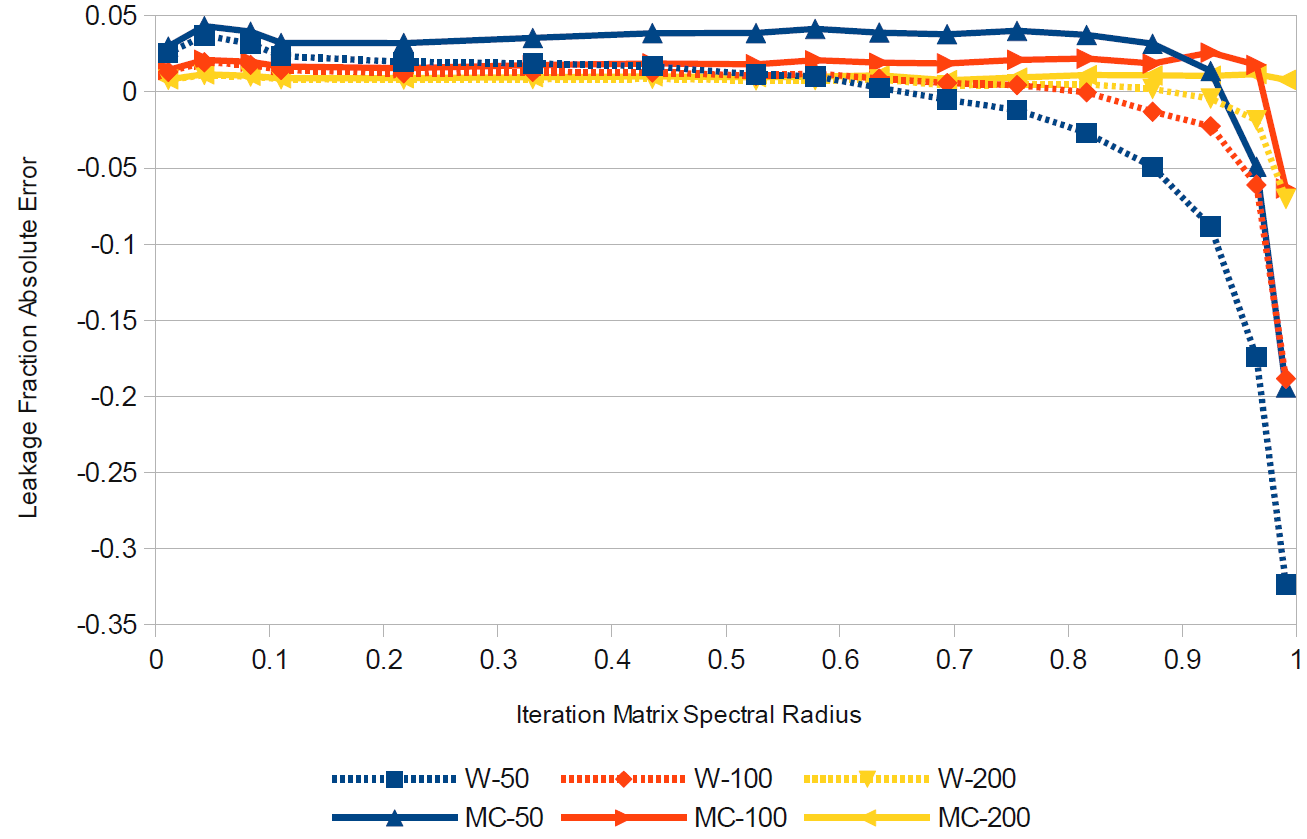
\includegraphics[width=5in,clip]{leakage_error.png}
  \end{center}
  \caption{\textbf{Measured and analytic domain leakage absolute error
      as a function of the iteration matrix spectral radius.}
    \textit{To test the behavior with respect to domain size, $n_i=50$
      (blue), $n_i=100$ (red), and $n_i=200$ (yellow) were used. The
      dashed lines represent the error using the Wigner rational
      approximation while the solid lines represent the error using
      the mean-chord approximation.}}
  \label{fig:measured_leakage}
\end{figure}

%%---------------------------------------------------------------------------%%
\section{Conclusion}
These relationships will serve as guidelines for selecting an
appropriate parallel algorithm strategy and provide a basis for
performance models for future parallel implementations of the adjoint
Neumann-Ulam method.

%%---------------------------------------------------------------------------%%
\pagebreak
\bibliographystyle{ieeetr}
\bibliography{references}
\end{document}


